\documentclass[final,12pt,3p,times,fleqn]{elsarticle}
\usepackage[utf8]{inputenc}
\usepackage[english]{babel}
\usepackage{amsmath,amsfonts,amssymb,graphicx,booktabs,hyperref,float,multirow}

\begin{document}

\begin{frontmatter}

\title{Power-Law Initialization for Budget-Constrained\\Physics-Informed Extreme Learning Machines}

\author[1,2]{Quang Nguyen\corref{cor1}}
\ead{nquang@hcmiu.edu.vn}

\address[1]{Department of Physics, International University, Ho Chi Minh City, Vietnam}
\address[2]{Viet Nam National University Ho Chi Minh City, Vietnam}

\cortext[cor1]{Corresponding author}

\begin{abstract}
Physics-Informed Extreme Learning Machines (PIELMs) solve linear PDEs in a single least-squares step, but their accuracy depends critically on the weight scale hyperparameter $R_m$. We propose power-law weight initialization, drawing weight magnitudes from $P(|w|) \propto |w|^{-\alpha}$, for sinusoidal-basis PIELMs. An ablation identifies the optimal range $\alpha \approx 0.75$--$1.25$, which spreads neurons across frequency decades rather than concentrating them in a narrow band. Through experiments on eight 1D and three 2D PDE benchmarks, we show: (i)~at tight neuron budgets ($h \leq 40$), power-law initialization outperforms Gaussian and uniform by up to $300\times$ in 1D; (ii)~the advantage \emph{amplifies} in 2D, exceeding $10^6\times$ at $h = 400$; (iii)~power-law degrades more gracefully when $R_m$ is misspecified. We recommend $\alpha = 1$ (log-uniform) as the default. All training uses PDE residuals and boundary conditions only.
\end{abstract}

\begin{keyword}
Physics-Informed Extreme Learning Machines \sep
Power-Law Initialization \sep
Sinusoidal Activation \sep
Spectral Basis Diversity
\end{keyword}

\end{frontmatter}


%% ===================================================================
\section{Introduction}
\label{sec:intro}
%% ===================================================================

Physics-Informed Neural Networks (PINNs)~\cite{raissi2019physics} embed PDE residuals into the training loss, enabling mesh-free solvers. However, PINNs require thousands of gradient-descent iterations and suffer from spectral bias---a preference for low-frequency components~\cite{rahaman2019spectral,wang2022pinns}.

Extreme Learning Machines (ELMs)~\cite{huang2006extreme} bypass iterative training: hidden weights are frozen at random and only output weights $\beta$ are solved analytically. Dwivedi and Srinivasan~\cite{dwivedi2020pielm} extended this to PDEs as Physics-Informed ELMs (PIELMs), solving a single linear system that enforces the PDE residual and boundary conditions.

A central limitation is sensitivity to the weight scale $R_m$. Dong~\cite{dong2022computing} showed that accuracy varies by orders of magnitude with $R_m$ and proposed differential evolution to find the optimum---an expensive search that partially negates the one-shot advantage. This sensitivity arises because standard initializations (Gaussian, uniform) concentrate weights in a narrow frequency band.

We address this through two ideas: (1)~\textbf{sinusoidal activation} for PIELM, following recent Fourier-based work~\cite{li2023fpielm,ren2025gffpielm,sitzmann2020siren}, making each neuron an explicit Fourier mode; and (2)~\textbf{power-law weight initialization} $P(|w|) \propto |w|^{-\alpha}$ with $\alpha \approx 1$, which spreads neurons across frequency decades. Tancik et al.~\cite{tancik2020fourier} explored log-uniform sampling ($\alpha = 1$) for deep Fourier feature networks and concluded that distribution shape does not matter. We show this conclusion does \emph{not} transfer to PIELMs: without iterative training to compensate, distribution shape becomes critical.

Our main findings are:
\begin{itemize}
    \item At tight neuron budgets ($h \leq 40$), power-law outperforms Gaussian by $10$--$300\times$ in 1D (Section~\ref{sec:neuron_budget}).
    \item The advantage \emph{amplifies} in 2D: Gaussian fails entirely ($L_2 > 0.6$) at $h = 400$ while power-law achieves $10^{-7}$, exceeding $10^6\times$ advantage (Section~\ref{sec:2d}).
    \item The optimal exponent is $\alpha \approx 0.75$--$1.25$; we recommend $\alpha = 1$ (log-uniform) as the default (Section~\ref{sec:alpha}).
    \item Power-law degrades gracefully when $R_m$ is misspecified (Section~\ref{sec:scale}).
\end{itemize}


%% ===================================================================
\section{Methods}
\label{sec:methods}
%% ===================================================================

\subsection{PIELM with Sinusoidal Basis}

Given a linear PDE $\mathcal{L}[u](x) = f(x)$ on $\Omega$ with Dirichlet conditions $u|_{\partial\Omega} = g$, PIELM approximates $\hat{u}(x) = \sum_{j=1}^{h} \beta_j \sin(w_j x + b_j)$, where $\{w_j, b_j\}$ are frozen and only $\beta$ is solved for. Because $\sin(\cdot)$ is an eigenfunction of differentiation, PDE operators have closed forms:
\begin{align}
    \text{Poisson } (-u'' = f): &\quad w_j^2 \sin(w_j x + b_j), \label{eq:poisson}\\
    \text{Helmholtz } (-u'' - k^2 u = f): &\quad (w_j^2 - k^2) \sin(w_j x + b_j). \label{eq:helmholtz}
\end{align}
For $d$-dimensional inputs with $\phi_j(\mathbf{x}) = \sin(\mathbf{w}_j^\top \mathbf{x} + b_j)$, the Laplacian gives $\|\mathbf{w}_j\|^2 \cdot \phi_j(\mathbf{x})$, so the formulation extends directly to 2D.

The PIELM system stacks PDE and boundary rows:
\begin{equation}\label{eq:system}
    \begin{bmatrix} A_{\text{pde}} \\ \lambda_{\text{bc}} A_{\text{bc}} \end{bmatrix} \beta =
    \begin{bmatrix} f_{\text{int}} \\ \lambda_{\text{bc}} g_{\text{bc}} \end{bmatrix},
\end{equation}
solved via $\beta = (A^\top A + \lambda I)^{-1} A^\top \mathbf{r}$ in one shot with cost $O(Nh^2 + h^3)$.

\subsection{Power-Law Initialization}

Standard initializations concentrate weights at a single scale: Gaussian $\mathcal{N}(0, R_m)$ clusters near zero; uniform $\mathcal{U}(-R_m, R_m)$ over-represents frequencies near $R_m$. We propose drawing weight magnitudes from a truncated power-law distribution:
\begin{equation}\label{eq:powerlaw}
    P(|w|) \propto |w|^{-\alpha}, \quad |w| \in [1, R_m],
\end{equation}
with random sign $\text{sgn}(w_j) \in \{-1, +1\}$ and bias $b_j \sim \mathcal{U}(-\pi, \pi)$. The exponent $\alpha$ controls the frequency allocation: $\alpha = 1$ gives log-uniform (equal probability per decade), $\alpha < 1$ favors higher frequencies, and $\alpha > 1$ favors lower frequencies. Our ablation (Section~\ref{sec:alpha}) identifies $\alpha \approx 0.75$--$1.25$ as optimal; we recommend $\alpha = 1$ as the default. In the language of power-law distributions~\cite{clauset2009powerlaw}, $\alpha = 1$ is the boundary between light-tailed and heavy-tailed regimes.

For sinusoidal activation, each neuron is a random Fourier feature~\cite{rahimi2007random,tancik2020fourier} whose frequency is $|w_j|$. Gaussian weights yield a narrowband kernel; power-law weights yield a broadband spectrum---a natural match for physical systems with multi-scale energy content.


%% ===================================================================
\section{Experimental Setup}
\label{sec:setup}
%% ===================================================================

All experiments use Eq.~\ref{eq:system} with $\lambda_{\text{bc}} = 100$, $\lambda = 10^{-10}$, double precision, and 20 seeds. 1D benchmarks use $N = 200$ interior points; 2D benchmarks use a $30 \times 30$ grid. The reference solution is used only for evaluation.

\paragraph{1D Benchmarks.}
(1)~Poisson: $u = \sin(\pi x)$;
(2)~Multi-frequency Poisson: $u = \sin(\pi x) + 0.3\sin(3\pi x) + 0.1\sin(7\pi x)$;
(3)~Helmholtz ($k{=}10$): $u = \sin(\pi x)e^{-4x^2}$;
(4)~High-frequency Poisson: $u = \sin(10\pi x)$;
(5)~Advection--diffusion ($\varepsilon{=}0.02$).
Additionally: (6)~Helmholtz $k{=}20$; (7)~$u = x(1{-}x^2)\sin(5\pi x)$; (8)~$u = \sin(\pi x)\cos(3\pi x)$.
All on $[-1,1]$ with $u(\pm 1) = 0$.

\paragraph{2D Benchmarks} on $[-1,1]^2$ with $u|_{\partial\Omega} = 0$:
(9)~Poisson: $u = \sin(\pi x)\sin(\pi y)$;
(10)~Multi-frequency: $u = \sin(\pi x)\sin(2\pi y) + 0.3\sin(3\pi x)\sin(\pi y)$;
(11)~Helmholtz ($k{=}5$): $u = \sin(\pi x)\sin(\pi y)$.

\paragraph{Initializations.}
Power-Law (proposed): $P(|w|) \propto |w|^{-\alpha}$ on $[1, R_m]$, $\alpha = 1$ (default), $b_j \sim \mathcal{U}(-\pi, \pi)$.
Gaussian: $w_j \sim \mathcal{N}(0, R_m)$, $b_j \sim \mathcal{N}(0, R_m)$.
Uniform: $w_j \sim \mathcal{U}(-R_m, R_m)$, $b_j \sim \mathcal{U}(-R_m, R_m)$.
Default: $R_m = 30$, $h = 400$.


%% ===================================================================
\section{Results}
\label{sec:results}
%% ===================================================================

\subsection{1D Benchmark at Fixed Scale}
\label{sec:benchmark}

Table~\ref{tab:benchmark} reports results at $h = 400$, $R_m = 30$. All initializations achieve $< 10^{-7}$ on the first three problems. Gaussian wins on high-frequency Poisson and advection--diffusion because $\mathcal{N}(0, 30)$ concentrates mass near the target frequency ($10\pi \approx 31.4$). This motivates the question: when the budget is \emph{tight}, does power-law's diversity become an advantage?

\begin{table}[htbp]
\centering
\caption{1D PIELM results (mean $\pm$ std, 20 seeds, $h{=}400$, $R_m{=}30$). Bold = best.}
\label{tab:benchmark}
\begin{tabular}{@{}llc@{}}
\toprule
\textbf{Problem} & \textbf{Init} & \textbf{Mean $L_2$ Error} \\
\midrule
\multirow{3}{*}{Poisson}
  & Power-Law & $\mathbf{7.9 \times 10^{-10}}$ \\
  & Gaussian    & $1.7 \times 10^{-8}$ \\
  & Uniform     & $1.1 \times 10^{-9}$ \\
\midrule
\multirow{3}{*}{Multi-Freq}
  & Power-Law & $\mathbf{2.0 \times 10^{-9}}$ \\
  & Gaussian    & $2.4 \times 10^{-8}$ \\
  & Uniform     & $3.7 \times 10^{-9}$ \\
\midrule
\multirow{3}{*}{Helmholtz}
  & Power-Law & $7.7 \times 10^{-9}$ \\
  & Gaussian    & $1.2 \times 10^{-7}$ \\
  & Uniform     & $\mathbf{5.3 \times 10^{-9}}$ \\
\midrule
\multirow{3}{*}{High-Freq}
  & Power-Law & $3.0 \times 10^{-5}$ \\
  & Gaussian    & $\mathbf{2.8 \times 10^{-7}}$ \\
  & Uniform     & $6.2 \times 10^{-6}$ \\
\midrule
\multirow{3}{*}{Adv-Diff}
  & Power-Law & $9.6 \times 10^{-4}$ \\
  & Gaussian    & $\mathbf{5.5 \times 10^{-6}}$ \\
  & Uniform     & $1.3 \times 10^{-2}$ \\
\bottomrule
\end{tabular}
\end{table}


\subsection{Neuron Budget Experiment}
\label{sec:neuron_budget}

We sweep $h \in \{20, 40, 60, 80, 100, 150, 200, 300, 400\}$ at fixed $R_m = 30$. Figure~\ref{fig:neuron_budget} shows the results.

\begin{figure}[htbp]
    \centering
    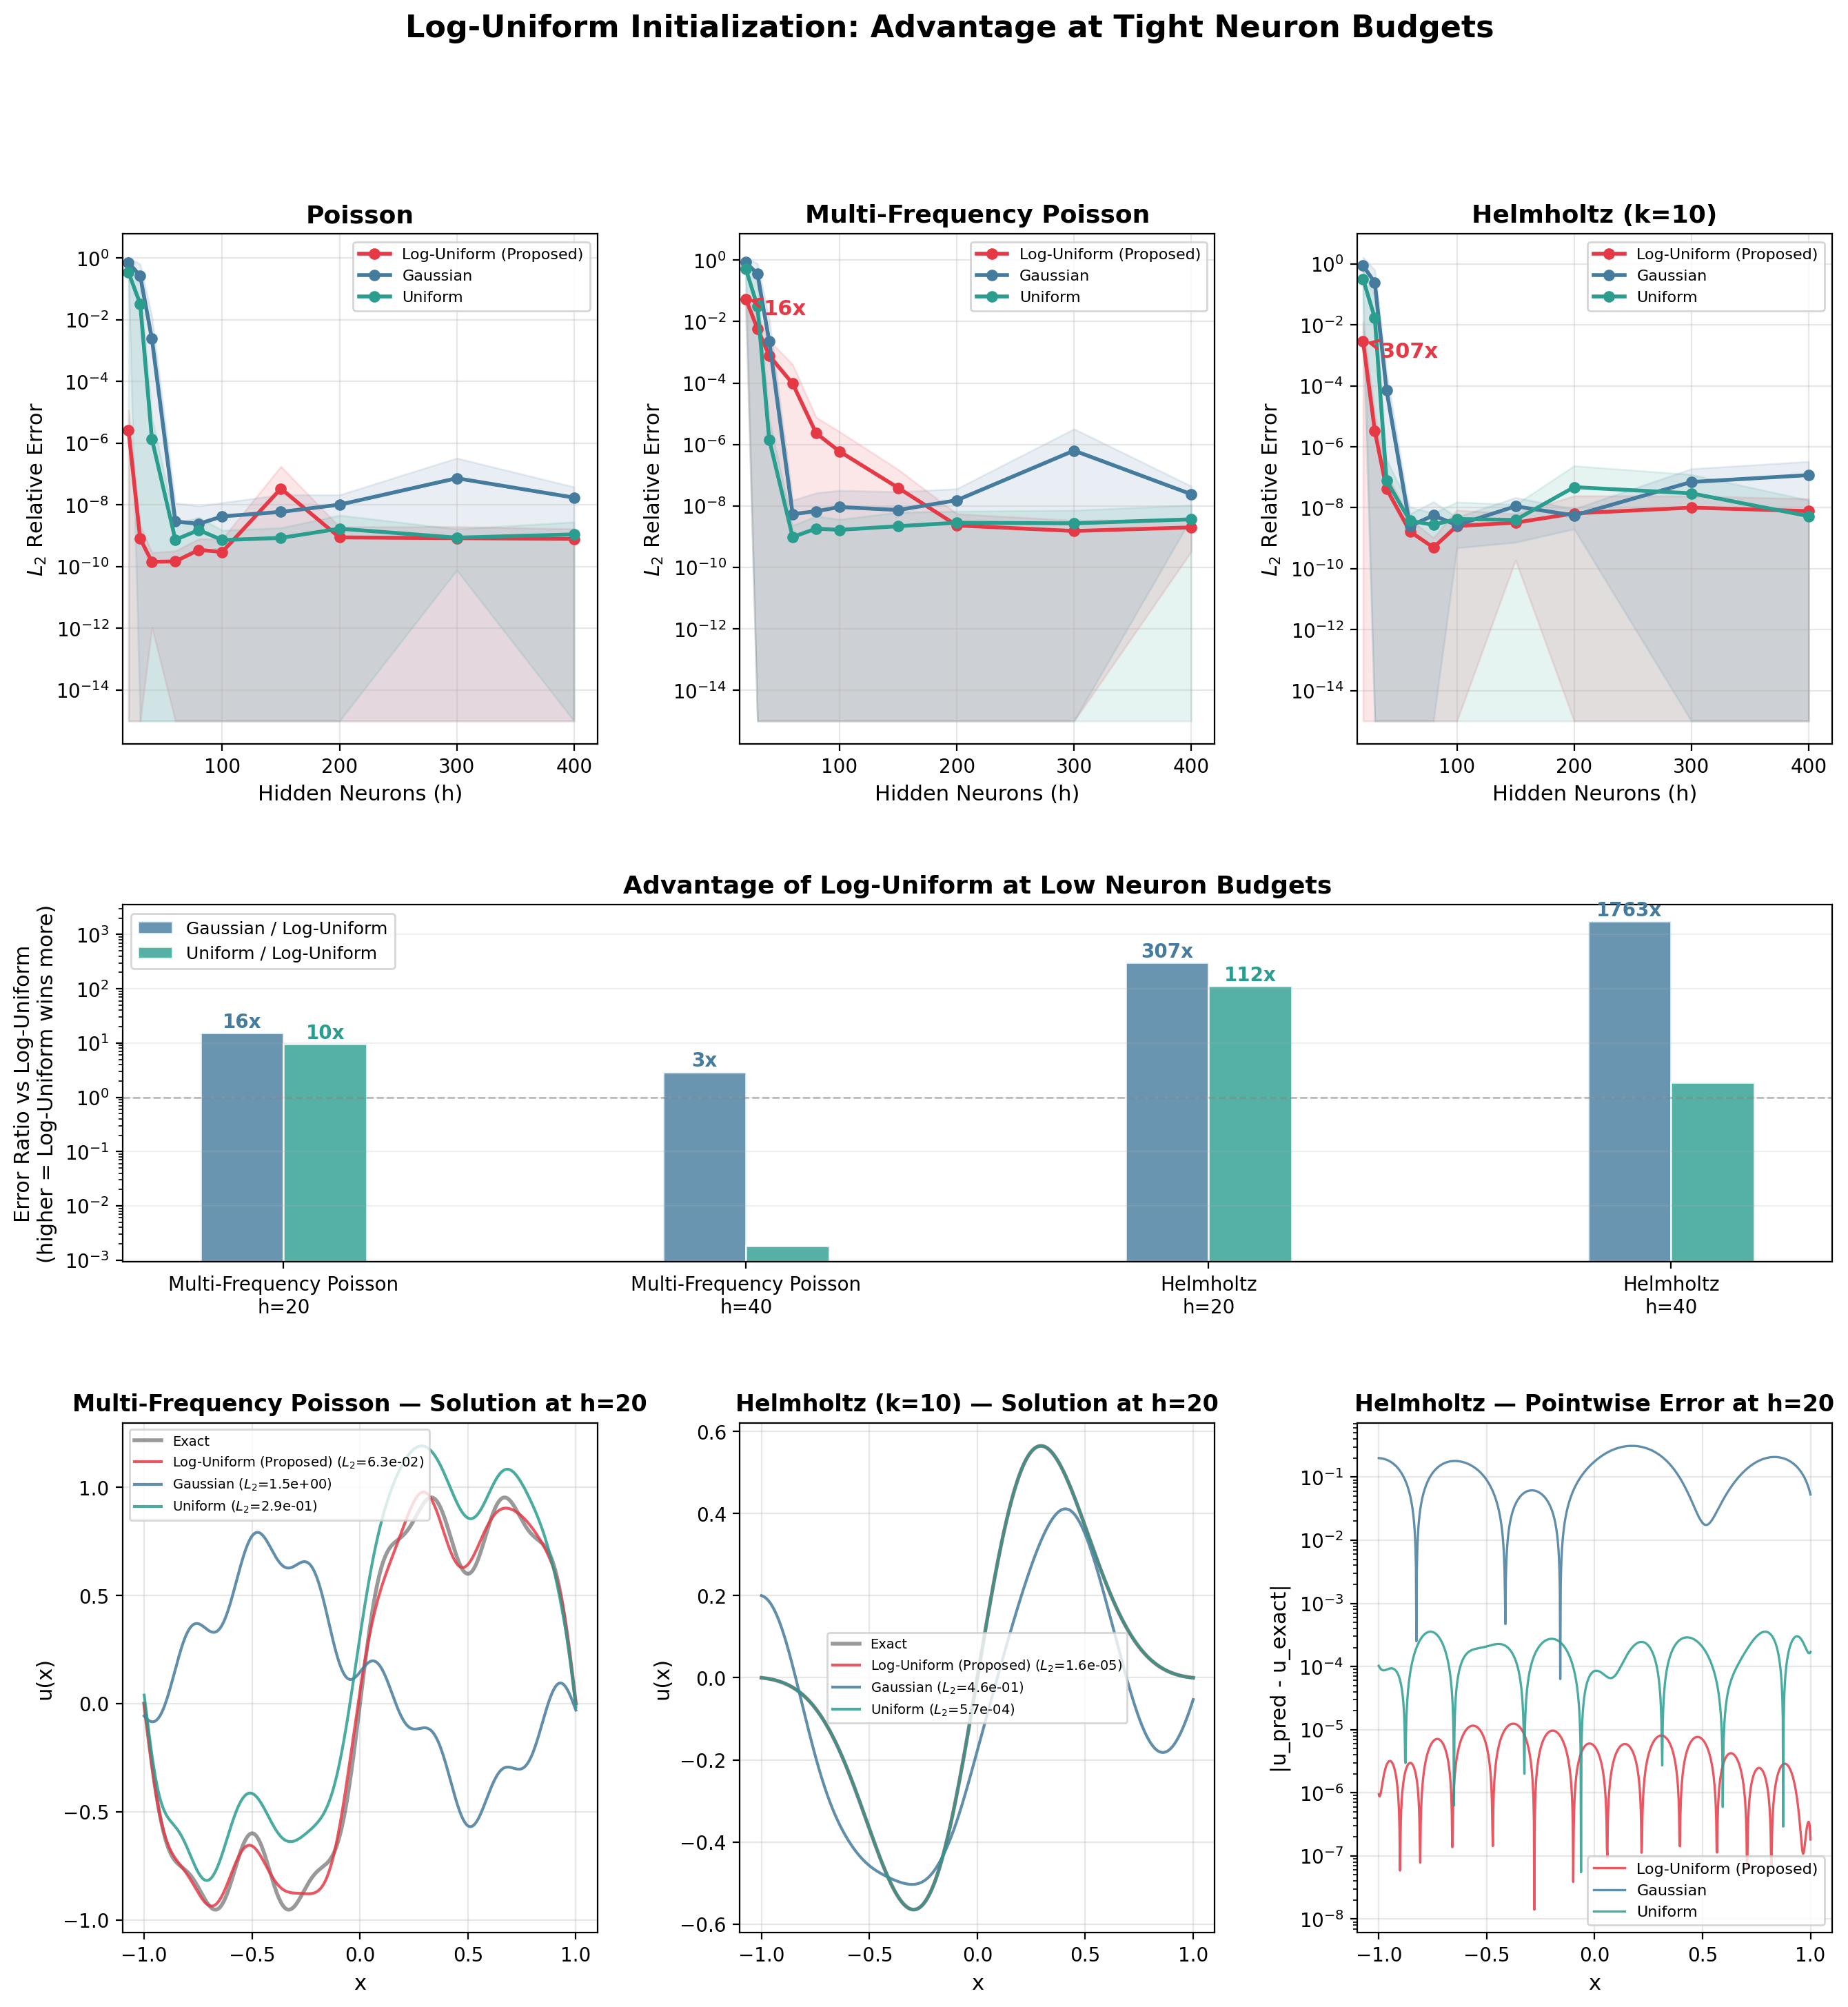
\includegraphics[width=\textwidth]{fig_neuron_budget_hero.png}
    \caption{\textbf{Power-law initialization at tight neuron budgets.} Top: $L_2$ error vs $h$ (shaded: $\pm 1$ std). Middle: Gaussian/power-law error ratio at $h = 20$ and $40$. Bottom: solution fields at $h = 20$; Gaussian and uniform fail while power-law tracks the exact solution.}
    \label{fig:neuron_budget}
\end{figure}

At $h = 20$, power-law achieves $L_2 = 2.9 \times 10^{-3}$ on Helmholtz while Gaussian fails ($8.9 \times 10^{-1}$)---a $300\times$ advantage. The mechanism: with 20 neurons, $\mathcal{N}(0, 30)$ produces many weights near $\pm 30$, creating nearly identical basis functions. Power-law distributes weights across $[1, 30]$ in log-space, ensuring each neuron covers a distinct frequency. As $h$ increases beyond 60, all methods converge.


\subsection{Power-Law Exponent Ablation}
\label{sec:alpha}

We sweep $\alpha \in \{0.5, 0.75, 1.0, 1.25, 1.5, 2.0, 3.0, 4.0\}$ at $h = 400$, $R_m = 30$. For single-frequency Poisson, $\alpha$ has little effect. For multi-frequency problems, accuracy spans eight orders of magnitude across the tested range: from $1.4 \times 10^{-9}$ at $\alpha = 0.75$ to $6.8 \times 10^{-2}$ at $\alpha = 2.0$ on multi-frequency Poisson. The optimal range $\alpha \approx 0.75$--$1.25$ corresponds to near-uniform allocation in log-space, balancing coverage across all frequency decades.


\subsection{Scale Robustness}
\label{sec:scale}

We sweep $R_m \in \{1, 2, \ldots, 150\}$ independently for each initialization (Figure~\ref{fig:scale}).

\begin{figure}[htbp]
    \centering
    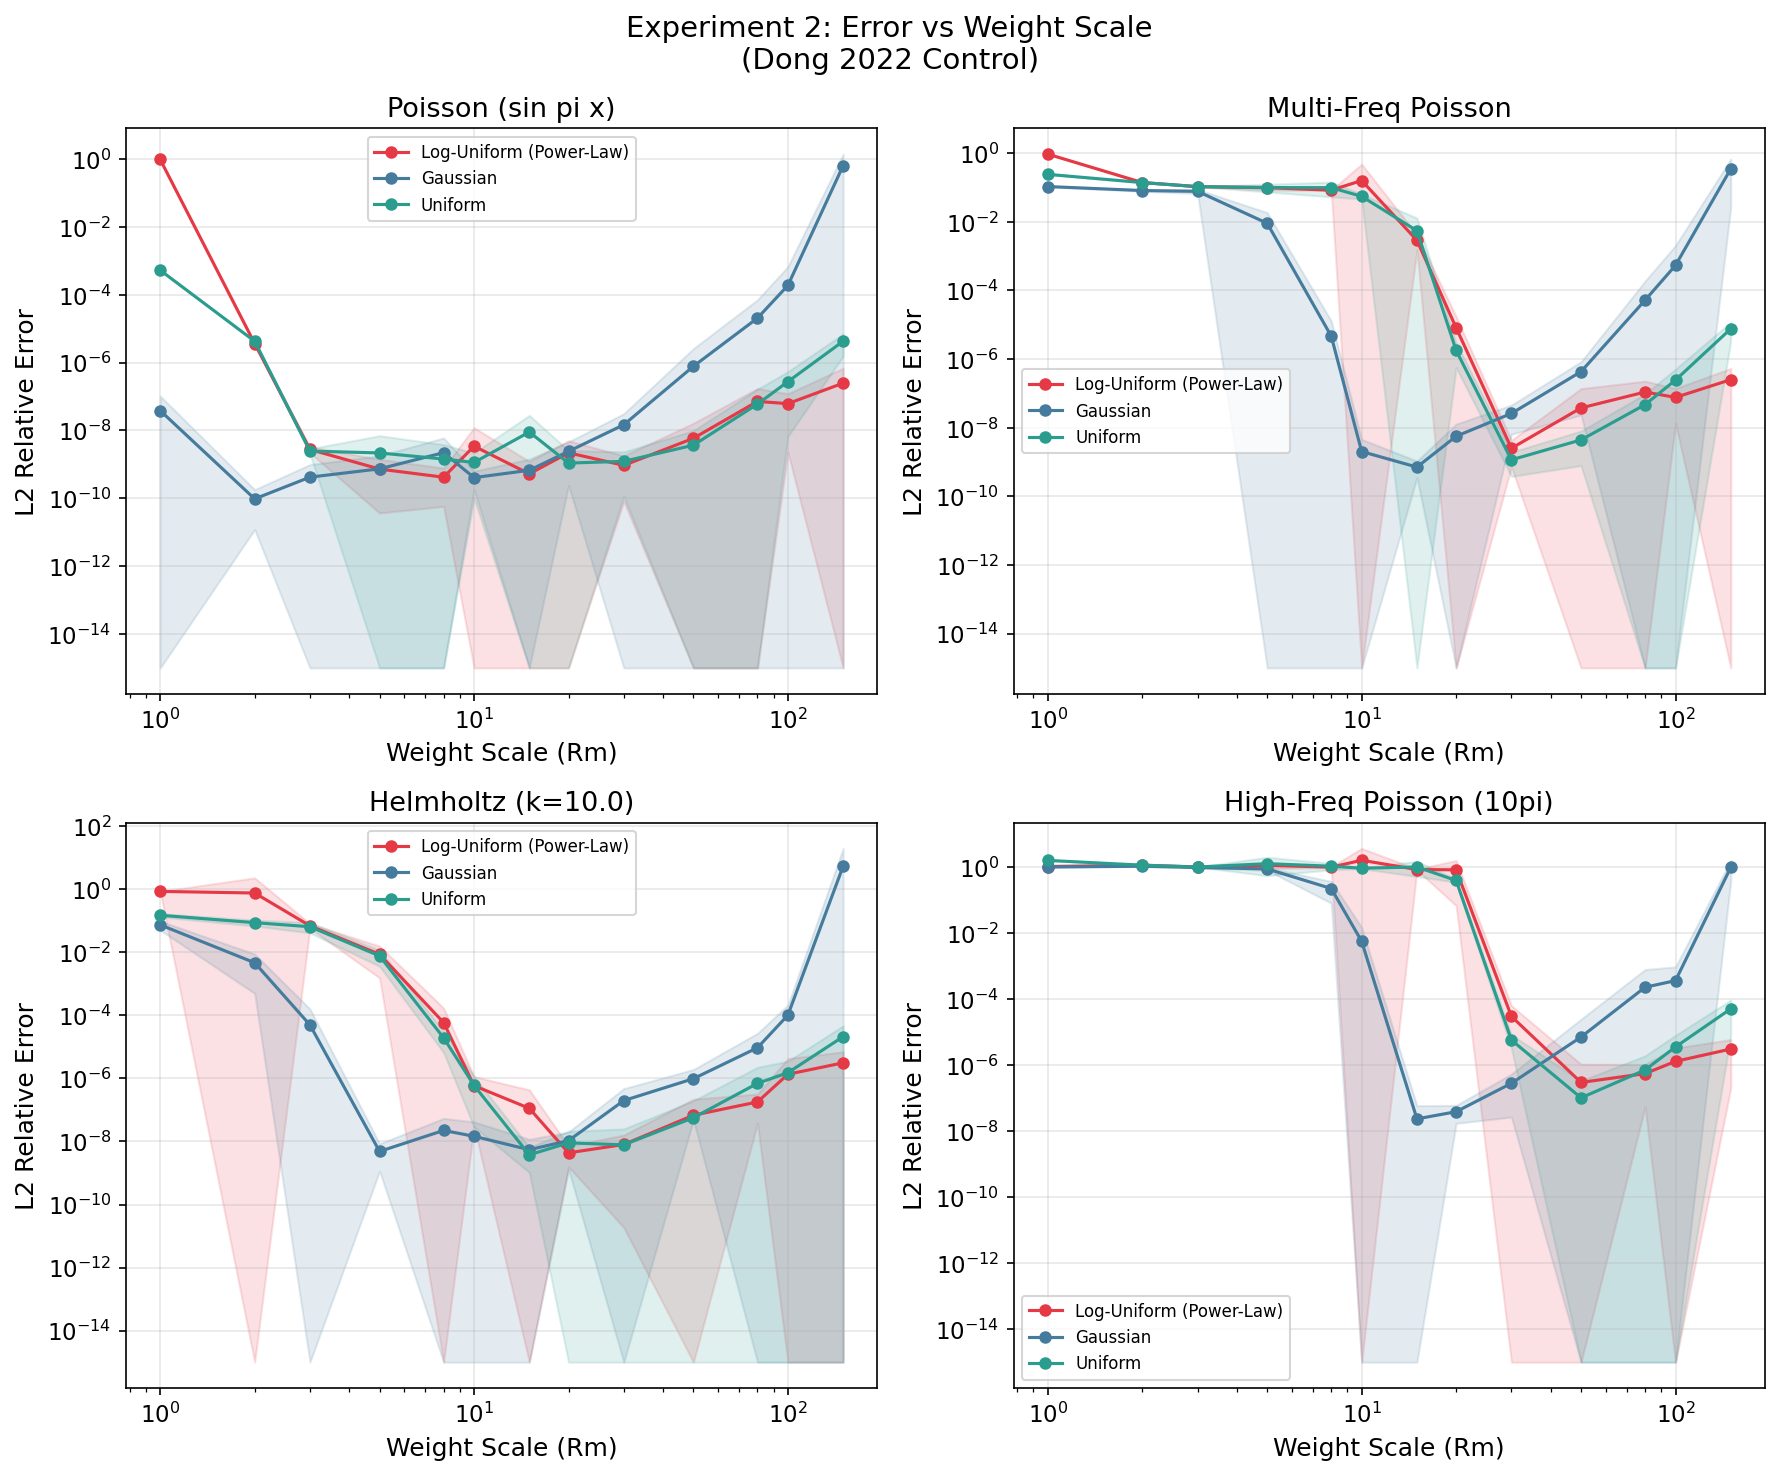
\includegraphics[width=\textwidth]{exp2_scale_sweep.png}
    \caption{$L_2$ error vs weight scale $R_m$ (shaded: $\pm 1$ std, 10 seeds). Gaussian degrades sharply when $R_m$ is over-specified; power-law remains robust.}
    \label{fig:scale}
\end{figure}

At optimal $R_m$, errors are comparable across initializations. However, degradation curves differ: at $R_m = 100$ on multi-frequency Poisson, Gaussian error $= 5.4 \times 10^{-4}$, power-law error $= 7.7 \times 10^{-8}$---a $7{,}000\times$ gap. Power-law provides a safe default when $R_m$ cannot be tuned per problem.


\subsection{Extension to Two Dimensions}
\label{sec:2d}

Table~\ref{tab:2d} reports 2D results at $h = 400$, $R_m = 30$.

\begin{table}[htbp]
\centering
\caption{2D PIELM results (mean, 20 seeds, $h{=}400$, $R_m{=}30$). Bold = best.}
\label{tab:2d}
\begin{tabular}{@{}lccc@{}}
\toprule
\textbf{Problem} & \textbf{Power-Law} & \textbf{Gaussian} & \textbf{Uniform} \\
\midrule
Poisson 2D              & $\mathbf{2.1 \times 10^{-7}}$ & $7.8 \times 10^{-1}$ & $6.0 \times 10^{-1}$ \\
Multi-Freq 2D           & $\mathbf{1.3 \times 10^{-4}}$ & $6.7 \times 10^{-1}$ & $4.7 \times 10^{-1}$ \\
Helmholtz 2D            & $\mathbf{8.9 \times 10^{-7}}$ & $9.5 \times 10^{-1}$ & $8.3 \times 10^{-1}$ \\
\bottomrule
\end{tabular}
\end{table}

The advantage is dramatically larger than in 1D: at $h = 400$---where 1D methods converge regardless of initialization---Gaussian and uniform \emph{fail completely} ($L_2 > 0.6$) on all three 2D benchmarks, while power-law achieves $10^{-4}$ to $10^{-7}$.

Figure~\ref{fig:2d_budget} shows the budget sweep. On Helmholtz 2D, Gaussian never drops below $L_2 = 0.96$ even at $h = 400$, while power-law reaches $6.8 \times 10^{-7}$---exceeding $10^6\times$.

\begin{figure}[htbp]
    \centering
    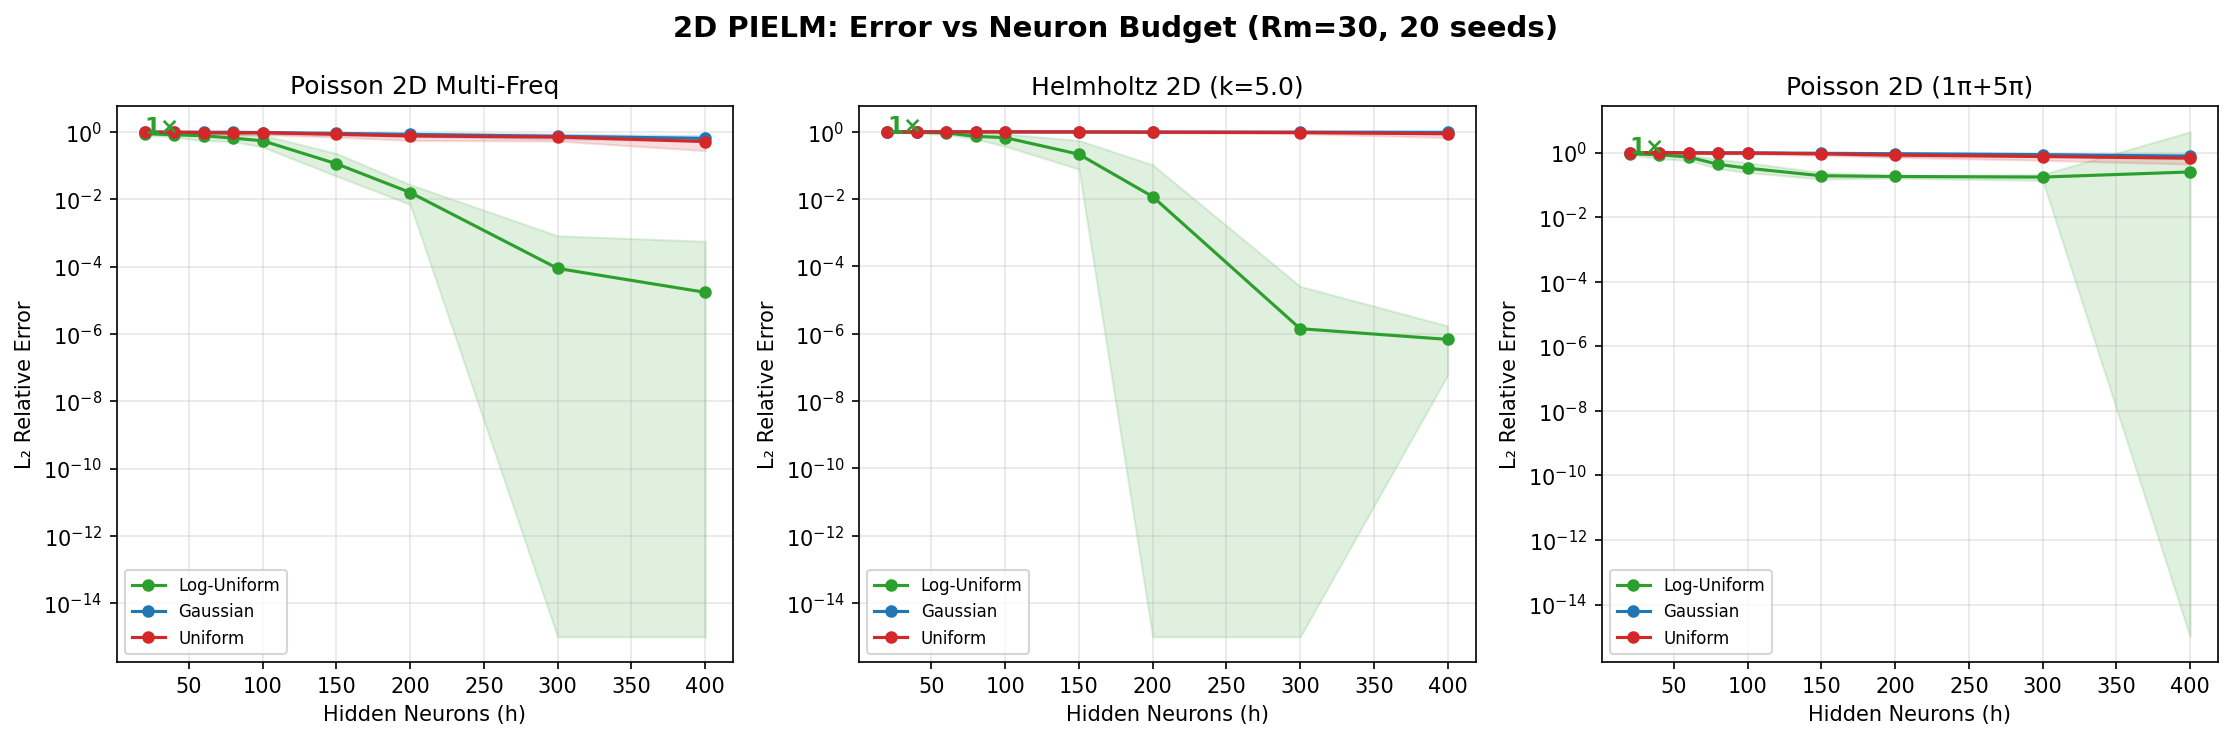
\includegraphics[width=\textwidth]{2d_neuron_budget.png}
    \caption{2D PIELM: $L_2$ error vs $h$ ($R_m{=}30$, 20 seeds). Gaussian and uniform fail even at $h = 400$; the advantage grows with $h$ rather than diminishing.}
    \label{fig:2d_budget}
\end{figure}

The mechanism is the same but amplified: Gaussian draws both components from $\mathcal{N}(0, R_m)$, so $\|\mathbf{w}_j\| \approx \sqrt{2}\,R_m$ is concentrated in a narrow band. Power-law distributes magnitudes across decades. In 2D, the waste from duplicate frequencies is more damaging---hence the larger advantage.


%% ===================================================================
\section{Discussion}
\label{sec:discussion}
%% ===================================================================

Our results delineate two regimes. When the system is over-parameterized ($h \gg$ required), all initializations achieve comparable accuracy and Dong's~\cite{dong2022computing} finding that scale matters more than distribution holds. When the budget is constrained ($h \leq 60$ in 1D, $h \leq 400$ in 2D), distribution shape becomes critical: power-law's frequency diversity produces a well-conditioned system, while Gaussian wastes capacity on redundant features. This is the regime where Tancik et al.'s~\cite{tancik2020fourier} conclusion---that only the standard deviation matters---breaks down, because there is no iterative training to compensate for a poor basis.

The 2D results reveal that this regime boundary shifts upward with dimensionality. Problems that are well-resolved at $h = 60$ in 1D require $h > 400$ in 2D for Gaussian, while power-law still solves them. This suggests the advantage will grow further in 3D.

\paragraph{Limitations.}
(1)~PIELM requires the PDE operator to be linear in $\beta$; nonlinear PDEs need iterative schemes.
(2)~When the solution contains a single high-frequency mode, Gaussian can be superior by concentrating neurons near the target frequency.
(3)~Global sinusoidal bases struggle with localized features (boundary layers); domain decomposition~\cite{dong2021extreme} may help.
(4)~Extension to 3D requires further study.


%% ===================================================================
\section{Conclusions}
\label{sec:conclusions}
%% ===================================================================

We proposed power-law weight initialization for sinusoidal-basis PIELMs. The main findings:
\begin{enumerate}
    \item At low neuron budgets, power-law outperforms Gaussian by up to $300\times$ in 1D by ensuring every neuron covers a distinct frequency scale.
    \item The optimal exponent is $\alpha \approx 0.75$--$1.25$, with $\alpha = 1$ (log-uniform) recommended as the default.
    \item Power-law degrades gracefully when $R_m$ is misspecified, reducing the need for per-problem tuning.
    \item In 2D, the advantage \emph{amplifies}: Gaussian and uniform fail entirely at $h = 400$ while power-law achieves $10^{-7}$, because 2D frequency space concentrates Gaussian weight magnitudes more tightly.
\end{enumerate}

These results position power-law PIELM as a practical choice for budget-constrained PDE solving. Future work will extend to 3D, nonlinear PDEs via iterative PIELM, and adaptive frequency allocation.


\appendix

\section{Solution Fields for Diverse Problem Types}
\label{app:diverse}

\begin{figure}[htbp]
    \centering
    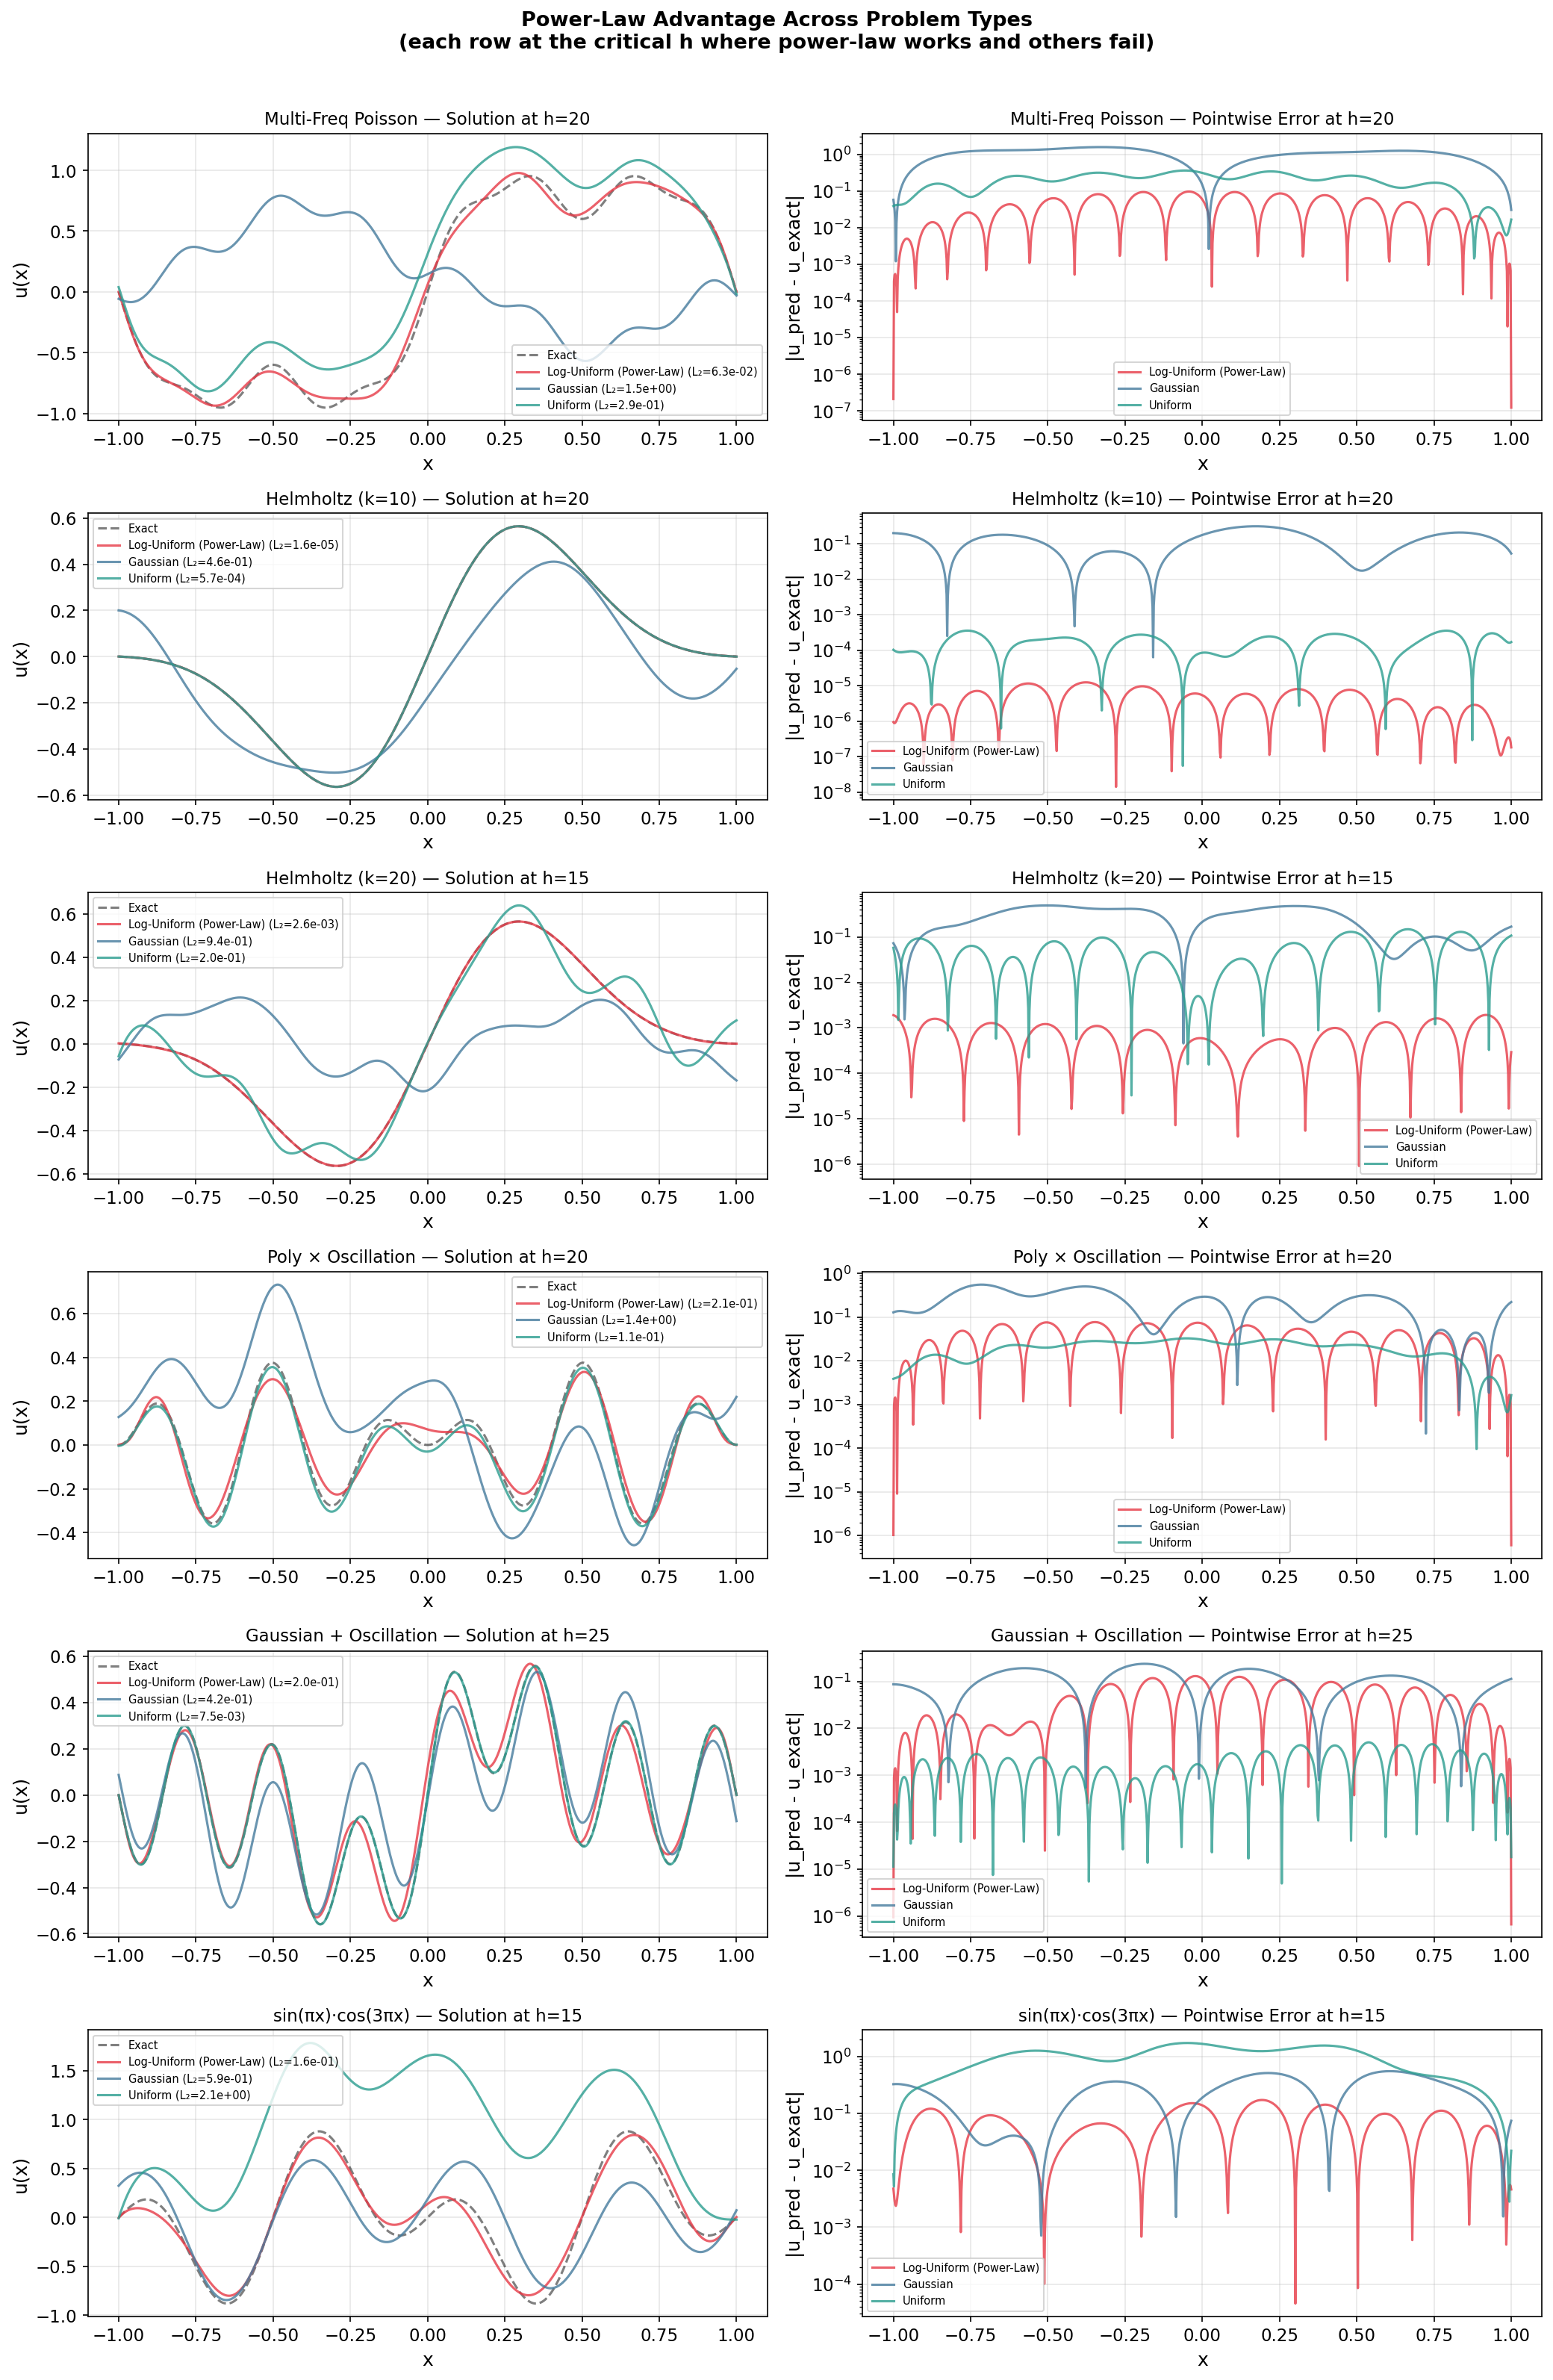
\includegraphics[width=\textwidth]{exp8_hero_diverse.png}
    \caption{\textbf{Power-law advantage across problem types.} Left: solutions; right: pointwise error. Rows 1--3 (Multi-Freq Poisson, Helmholtz $k{=}20$ at $h{=}20$ and $h{=}15$): power-law tracks the exact solution while others fail. Rows 4--5 (Poly $\times$ Oscillation, Gaussian + Oscillation): all methods struggle, but power-law degrades more gracefully. Row 6 ($\sin(\pi x)\cos(3\pi x)$ at $h{=}15$): power-law resolves the product structure.}
    \label{fig:diverse}
\end{figure}


\bibliographystyle{elsarticle-num}
\bibliography{references}

\end{document}
